\documentclass[letter paper]{article}
\usepackage[left=22mm, top=28mm, right=30mm, bottom=22mm]{geometry}
\usepackage[croatian]{babel}
\usepackage{enumerate}
\usepackage{outlines}
\usepackage[T1]{fontenc}
\usepackage[utf8]{inputenc}
\usepackage{fancyhdr}
\usepackage{graphicx}
\usepackage{amsmath}
\usepackage{amssymb}
\usepackage{fix-cm}
\usepackage{color}
\usepackage{colortbl}
\usepackage{multirow}
\usepackage{array}
\usepackage{tikz}
\usepackage{pgfplots}
\usetikzlibrary{arrows,shapes,automata,backgrounds,petri,patterns,shadows,fadings,calc,decorations,decorations.text}
\usetikzlibrary{calc} 
\usepackage[european]{circuitikz}
\usepackage{calc}
\usepackage[shadow,color=mc1,linecolor=mc1,bordercolor=black,textwidth=24mm]{todonotes}
\usepackage{tikz}
\usetikzlibrary{circuits.logic.US} 
\usepackage{pdfpages}
\usepackage{circuitikz}
\usepackage{embedfile}
\usepackage{hyperref}
\hypersetup{
    colorlinks,
    citecolor=black,
    filecolor=black,
    linkcolor=black,
    urlcolor=black,
}


\definecolor{mc1}{RGB}{	186,186,235}

\setlength{\headheight}{13pt}
\fancypagestyle{pahuljica_stil}
{
\lhead{\small\sc{Aljukić Adisa}} \chead{} \rhead{\includegraphics[scale=0.65,trim=4mm 4mm 4mm 4mm,clip=true]{pahuljica.pdf}}
\lfoot{} \cfoot{\thepage} \rfoot{}
\renewcommand{\headrulewidth}{0.45pt}
\renewcommand{\footrulewidth}{0pt}
}
\newcommand{\newsize}[1]{\color{black}\fontsize{8pt}{10pt}\selectfont{#1}}
\newcommand{\newtodo}[1]{\todo{\newsize{#1}}}

\begin{document}
\noindent Univerzitet u Tuzli \hfill ZIMA 2015 \\
Fakultet elektrotehnike \hfill Aljukić Adisa \\
Tehnologije za podršku tehničkom pisanju 

\vspace{5mm}
\begin{center}
 \LARGE {\textsc{Druga Zadaća iz Predmeta Tehnologije za Podršku Tehničkom Pisanju}\newtodo{Naslov dokumenta vertikalno je pomjeren za 5mm u odnosu na prethodni i naredni sadržaj.}}\\ 
\end{center}

\vspace{5mm}

\begin{abstract}
U okviru zadaće II biti će demonstrirano svo stečeno znanje iz predmeta Tehnologije za podršku tehničkom pisanju vezano za \LaTeX.~ Studenti će demonstrirati stečeno znanje na način da repliciraju sadržaj dokumenta(stranice od 1 do 4) pri čemu moraju obratiti pažnju na svaki detalj u orginalnom dokumentu. Replicirani dokument mora biti vjerodostojna kopija orginalnom dokumentu(100\% kopija osim dijela prezime i ime.  Kako rezultat, studenti će predati kod prema pravilima definiranim na prethodnoj stranici teksta zadaće.
\end{abstract}

\tableofcontents
\listoffigures
\listoftables

\section{Stil dokumenta}

\subsection{Margine dokumenta}
Margine stranice dokumenta postavljene su na sljedeći način: lijeva i donja na 22 mm, desna na 30 mm i gornja na 28mm. Na mjesto \textsl{Prezime Ime} upisat vaše prezime i ime. Obratiti pažnju da se na tekućoj stranici dokumenta zadaće, ne nalazi zaglavlje i podnožje. U okviru zadaće korisiti \LaTeX komande i okruženja samo na mjestima gdje to ima smisla.

\newpage

\pagestyle{pahuljica_stil}

\subsection{Zaglavlje i podnožje dokumenta}
Stil dokumenta generirati sa komandama iz oaketa \texttt{fancyhdr} pri čemu će se novi stil zvati \texttt{pahuljica\_stil}. Slika unutar zaglavlja stranice dokumenta (\textsl{pahuljica.pdf} ),  skalirana je na 0.65 a prostor oko slike skraćen je za 4 mm sa svih strana.\newtodo{Upotrijebiti \texttt{trim} \& \texttt{clip} opcije}~ Debljina linije u zaglavlju je 0.45 pt.

\section{Matematički mod i tabele}

\subsection{Matematički mod}
Tokom semestra, u \LaTeX-u smo upoznali matematički mod\footnote{Ne zaboravite da matematički mod zahtjeva uključenje paketa amsmath.} koji nam omogućava i formatiranje matrica

\begin{displaymath}
\left|
\left[
\begin{matrix}

2 & 1 & 1\\
-1& 1 & 4\\
0 & 3 & 1 \\
\end{matrix}
\right]
\left[
\begin{matrix}

0 & 1 & 1\\

3 & -1 & 0\\

5 & -2 & 1\\
\end{matrix}
\right]
\right|
=
\left|
\begin{matrix}

8  & -1  & 3\\
23 & -10 & 3\\
14 & -5  & 1\\
\end{matrix}
\right|
=
96
\end{displaymath}

\noindent U nastavku imamo primjer jedne diferencijalne jednačine drugog reda
\begin{equation}
x^2\frac{d^2B_{n,m}^{(\alpha,\beta)} (x)}{dx^2}+[(\alpha+2)x+\beta]\frac{dB_{n,m}^{(\alpha,\beta)}(x)}{dx}-[n(\alpha+n+1)+\frac{m\beta}{x}]B_{n,m}^{(\alpha,\beta)}(x)=0
y(t)=e^{-\beta t}sin(\omega_0 t + \frac{\theta}{2})

\end{equation}


\noindent Web adresa Fakulteta elektrotehnike Univerziteta u Tuzli je  

\fontfamily{ptm}{\fontsize{90pt}{90pt}\selectfont{\href{http://www.fet.ba/}{www.fet.ba}}}


\normalsize{}



\noindent U prethodnom redu, visina teksta je \textsl{90 pt}\footnote{Obratiti pažnju da će nam trebati paket \texttt{fix-cm}} a familija fonta je \textit{Times.}


\subsection{Tabele}

U nastavku imamo tri table postavljene jedna pored druge koristeći okruženje \texttt{\color{blue}minipage\color{black}, \color{blue} tabular \color{black}i \color{blue} table.}



\begin{table}[h]

\renewcommand{\arraystretch}{1.3}

\begin{minipage}[b]{0.33\textwidth}


\centering
\begin{tabular} {c c}
\hline \hline
Bodovi & Ocjena \\ \hline
94 - 100 & 10 \\
84 - 93 & 9\\
74 - 83 & 10 \\
64 - 73 & 9 \\
54 - 63 & 10 \\
\hline
\end{tabular}
\caption{Bodovi i ocjene}
\label{tabela:tab1}
\end{minipage}
{}
\begin{minipage}[b]{0.33\textwidth}
\centering
\begin{tabular} {c c}
\hline \hline
\rowcolor[RGB]{77,77,77}\color{white}Bodovi & \color{white}Ocjena \\ \hline
94 - 100 & 10 \\
\rowcolor[RGB]{235,229,229}84 - 93 & 9\\
74 - 83 & 10 \\
\rowcolor[RGB]{235,229,229}64 - 73 & 9 \\
54 - 63 & 10 \\
\hline \hline
\end{tabular}
\caption{Bodovi i ocjene}
\label{tabela:tab2}
\end{minipage}
{}
\begin{minipage}[b]{0.33\textwidth}
\centering
\begin{tabular} {|l|c|r|}
\hline \hline 
 \cellcolor[RGB]{204,255,204}L1 & L2 & L3 \\ \cline{3-3}
  \multicolumn{2}{c}{\cellcolor[RGB]{204,204,255}MC1}\vline & \multirow{2}{*}{MR1}  \\ \cline{1-2}
  A & B &  \\ \hline
  \multirow{2}{*}{MR2} & \multicolumn{2}{c}{MC2} \vline \\ \cline{2-2}
   & D & \cellcolor[RGB]{255,229,204} E \\ \hline
  G & \cellcolor[RGB]{255,204,204}E & M \\ \hline \hline

\end{tabular}
\caption{Spajanje ćelija}
\label{tabela:tab3}
\end{minipage}
\end{table}

\begin{center}

\fbox{\colorbox{pink}{\parbox{80mm}{U nastavku prikazana je lista malih Grčkih karaktera
\begin{enumerate}[a)]
\item $\alpha$, $\Delta$,$\sigma$,$\Gamma$,$\rho$,$\Psi$,
\item $\mu$, $\gamma$, $\epsilon$, $\Omega$, $\psi$, $\pi$,
\item $\kappa$, $\theta$, $\delta$, $\omega$, $\lambda$, $\tau$
\end{enumerate}
}}}
\end{center}

\newpage


\section{Paketi za crtanje u \LaTeX-u}

\subsection{TikZ paket}

Na slici 1 prikazana je serija složenih funkcija oblika $y=ax^2-3x+cos(90x)$ kreiranih sa okruženjem \texttt{\color{blue}tikzpicture} \color{black}i \texttt{\color{blue}axis} \color{black}. Serija funkcija nacrtana je za opseg vrijednosti $a=\{-2.4,-2.1,...,2.4\}$. Za crtanje  koristiti komandu \texttt{ \textcolor{red}{\textbackslash addplot}\{\} } u sklopu komande \texttt{ \textcolor{red}{\textbackslash foreach}\{\} } koja ima varijablu \textbf{a} koja se mijenja u skladu sa prethodno definiranim opsegom i korakom.Za aktiviranje mrežice na grafiku koristiti opciju \texttt{grid} a za postavku opsega grafika (\textit{plot-a}) koristiti opcije \texttt{xmin=-5, xmax=5, ymin=-20, ymax=20} u okviru \color{blue}axis \color{black} okruženja.Za skaliranje diagrama na slikama 1 i 2 koristiti opciju \texttt{scale} u okviru okruženja \color{blue}\texttt{tikzpicture} \color{black}.



\begin{figure} [h]
	\begin{minipage}{0.5\textwidth}
		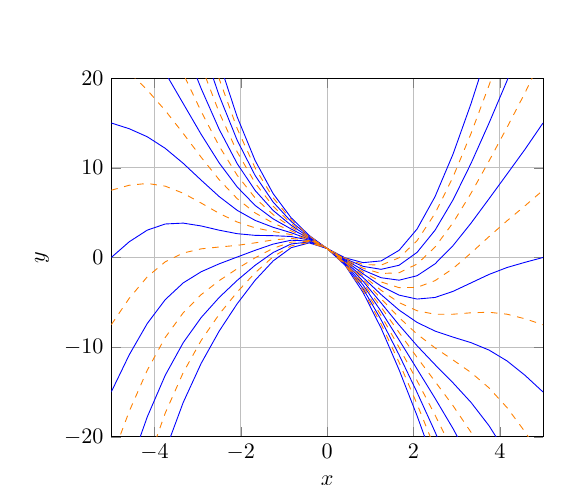
\begin{tikzpicture}[scale=0.8]
		\begin{axis}	 [grid, xmin=-5,xmax=5,ymin=-20,ymax=20, xlabel=$x	$,ylabel=$y$]		
		\foreach \a in{-2.4,-1.8,...,2.4}{
		\addplot[blue]
		expression{\a*x^2 -3*x + cos(90*x)};}
		\foreach \a in{-2.1,-1.5,-0.9,-0.3,0.3,0.9,1.5,2.1}{
		\addplot[orange,dashed]
		expression{\a*x^2 -3*x + cos(90*x)};}
		\end{axis}
		\end{tikzpicture}
		\caption{Serija složenih funkcija}
	\end{minipage}
				{}
	\begin{minipage}{0.5\textwidth}
		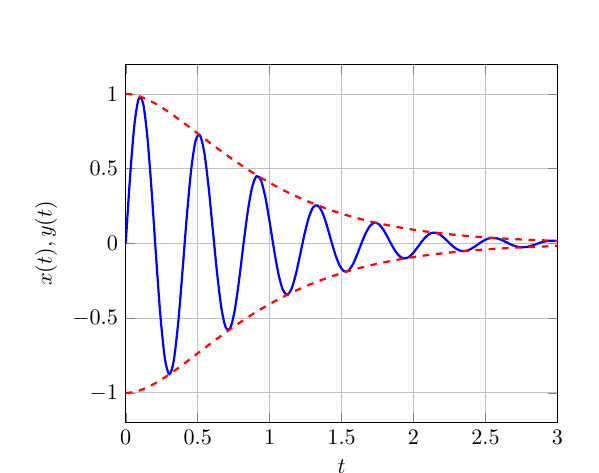
\begin{tikzpicture}[scale=0.8]
		\begin{axis}	[grid, xmin=0,xmax=3,ymin=-1.2,ymax=1.2,xlabel=$t$,ylabel=${x(t), y(t)}$]
		\addplot[blue,line width=1pt,smooth] plot[domain= 0:3, samples=100]
		expression{(1+2*x)*exp(-2*x)*sin(280*3.14*x)};
		\addplot[red,line width=1pt,dashed] plot[domain= 0:3, samples=100]
		expression{(1+2*x)*exp(-2*x)};
		\addplot[red,line width=1pt,dashed] plot[domain= 0:3, samples=100]
		expression{-(1+2*x)*exp(-2*x)};
		\end{axis}
		\end{tikzpicture}
		\caption{\textit{Damping} sinusne funkcije}
	\end{minipage}	
\end{figure}

\noindent Na slici 2 prikazane su sljedeće funkcije

\begin{equation}
	x(t)=(1+2t)e^{-2t}\sin(280 \pi t)
	\end{equation}
	\begin{equation}
	y(t)=\pm(1+2t)e^{-2t} 
	\end{equation}
	

\noindent  \textit{Gauss}-ova funkcija greške definirana je kao


\begin{equation*}
	erf(x)=\frac{2}{\sqrt{\pi}}{\int_0^x} e^{-t^2}\,dt
\end{equation*}


\noindent Prethodni integral ne možemo analitički riješiti ali zato možemo sljedeći

\begin{equation*}
I= \int_{0}^{\frac{a}{2}} \, \frac{dx}{\sqrt{a^2-x^2}}=arcsin{\left(\frac{x}{a}\right)}\bigg|_0^\frac{a}{2}=\frac{\pi}{6}
\end{equation*}
\noindent Sistem jednačina zapisanih prema \textit{Kirchoff}-ovim zakonima, za neko električno kolo je
\begin{align}
i_1-i_2-i_3&=0 \\ 
\nonumber -R_2i_2+ \mathcal{E}_1-R_1i_1&=0 \\
\nonumber -R_3i_3- \mathcal{E}_2- \mathcal{E}_1 + R_2i_2&=0 \\
\nonumber
\end{align}


\newpage


\subsection{Električne sheme i \texttt{\color{red}circuitikz} paket}
Na slici 3 prikazana je logička shema 74HC153 multiplexera.\footnote{Prilikom crtanja logičke šeme neophodno je uključiti tikz biblioteku \textit{circuits.logic.US}}. Ukoliko imate poteškoća sa realizacijom logičke i električne sheme možete se poslužiti primjerima iz kratkog uputstva \texttt{circutikz} paketa, koje se nalazi na CTAN \href{http://texdoc.net/show.php?pkg=circuitikz}{\color{cyan}{stranici}}.

\begin{figure}[ht!]
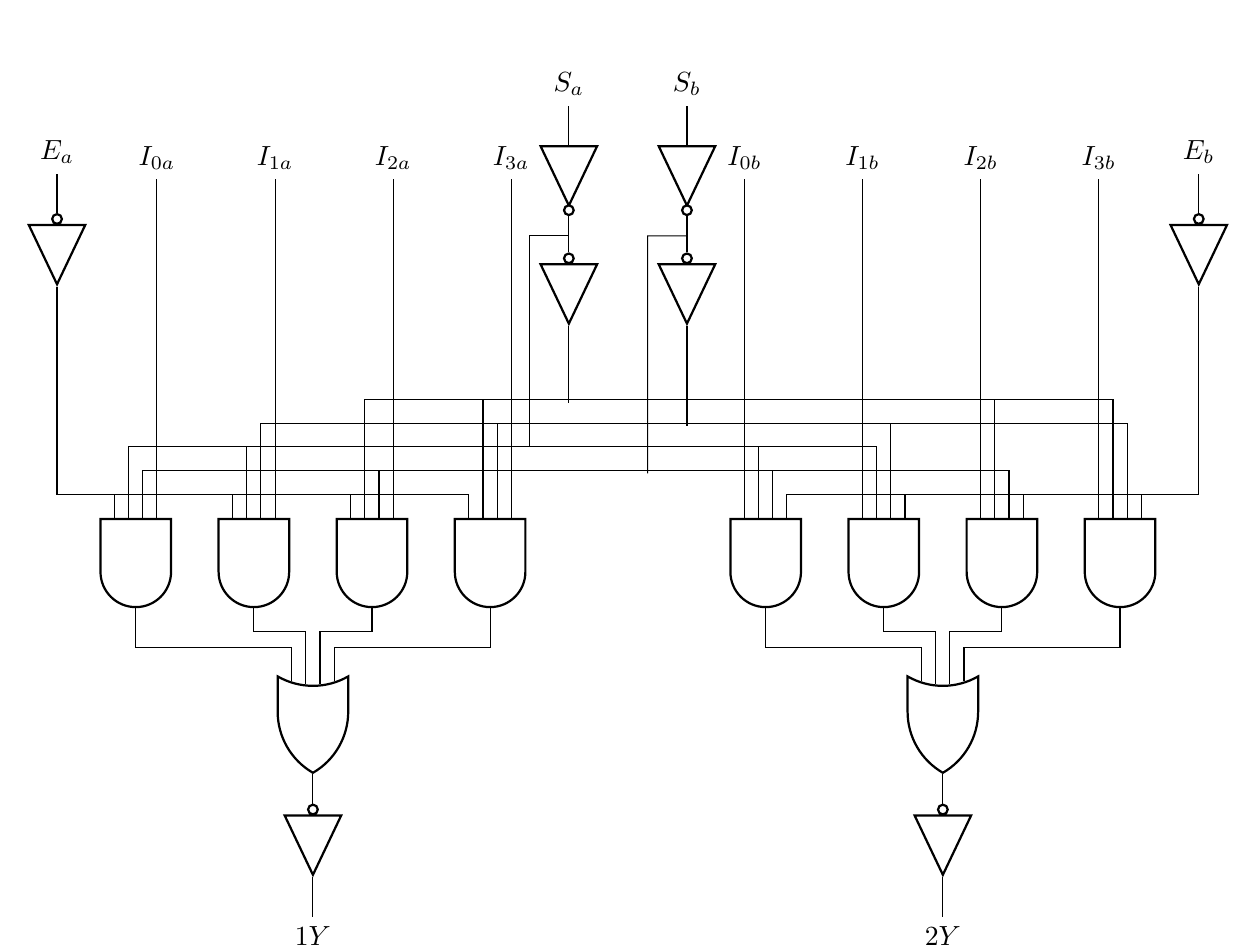
\begin{tikzpicture}[circuit logic US, every circuit symbol/.style={thick}]

	\node[buffer gate, point down,inputs={i}] (buf1) at (-1,3)    {}; 
	\node[and gate,inputs={nnnn}, point down] (and1) at (0,-1)    {};
	\node[and gate,inputs={nnnn}, point down] (and2) at (1.5,-1)  {};
	\node[and gate,inputs={nnnn}, point down] (and3) at (3,-1)    {};
	\node[and gate,inputs={nnnn}, point down] (and4) at (4.5,-1)  {};
	\node[or gate,inputs={nnnn}, point down]  (or1)  at (2.25,-3) {};
	\node[not gate, point down]               (not1) at (5.5,4)   {}; 
	\node[buffer gate, point down,inputs={i}] (buf2) at (5.5,2.5) {};
	\draw (buf1.output) -- ++(down:26.4mm) -| (and1.input 4);
	\draw (and1.output) -- ++(down:5mm) -| (or1.input 4);
	\draw (and2.output) -- ++(down:3mm) -| (or1.input 3);
	\draw (and3.output) -- ++(down:3mm) -| (or1.input 2);
	\draw (and4.output) -- ++(down:5mm) -| (or1.input 1);
	\draw (not1.output) -- (buf2.input);
	\node[not gate, point down] (not2) at (7,4) {}; 
	\node[buffer gate, point down,inputs={i}] (buf3) at (7,2.5)    {};
	\node[buffer gate, point down,inputs={i}] (buf4) at (13.50,3)  {}; 
	\node[and gate,inputs={nnnn}, point down] (and5) at (8,-1)     {};
	\node[and gate,inputs={nnnn}, point down] (and6) at (9.5,-1)   {};
	\node[and gate,inputs={nnnn}, point down] (and7) at (11,-1)    {};
	\node[and gate,inputs={nnnn}, point down] (and8) at (12.5,-1)  {};
	\node[or gate,inputs={nnnn},  point down] (or2)  at (10.25,-3) {};
	\draw (not2.output) -- (buf3.input);
	\draw (buf4.output) -- ++(down:26.4mm) -| (and8.input 1);
	\draw (and5.output) -- ++(down:5mm) -|  (or2.input 4);
	\draw (and6.output) -- ++(down:3mm) -|  (or2.input 3);
	\draw (and7.output) -- ++(down:3mm) -|  (or2.input 2);
	\draw (and8.output) -- ++(down:5mm) -|  (or2.input 1);
	\draw (buf1.input) -- ++(up:5mm) node [above]{$E_a$};
	\draw (buf4.input) -- ++(up:5mm) node [above]{$E_b$};
	\draw (not1.input) -- ++(up:5mm) node [above]{$S_a$};
	\draw(not2.input) -- ++(up:5mm) node [above]{$S_b$};
    \draw(and1.input 1) -- ++(up:4.3) node [above]{$I_{0a}$}; 
	\draw (and2.input 1) -- ++(up:4.3) node [above]{$I_{1a}$};
	\draw (and3.input 1) -- ++(up:4.3) node [above]{$I_{2a}$};
	\draw(and4.input 1) -- ++(up:4.3) node [above]{$I_{3a}$};
	\draw (and5.input 4) -- ++(up:4.3) node [above]{$I_{0b}$}; 
	\draw (and6.input 4) -- ++(up:4.3) node [above]{$I_{1b}$};
	\draw (and7.input 4) -- ++(up:4.3) node [above]{$I_{2b}$};
	\draw (and8.input 4) -- ++(up:4.3) node [above]{$I_{3b}$};

	\draw (not1.output) -- ++(down:2.5mm)
	      -- ++(left:5mm) -- (5,0.45);
	\draw (not1.output) -- (buf2.input);
	\draw (not2.output) -- ++(down:2.5mm) -- ++(left:5mm)
	      -- (6.5,0.1);
	\draw(not2.output) -- (buf3.input);

	\draw(buf2.output) -- (5.5,1);
	\draw(buf3.output) -- (7,0.7);
	\draw (and1.input 4) -- ++(up:3mm)  -| (and2.input 4)
	      -- ++(up:3mm) -|    (and3.input 4) -- ++(up:3mm)  -| (and4.input 4);
	\draw (and5.input 1) -- ++(up:3mm)  -| (and6.input 1)
	      -- ++(up:3mm) -|    (and7.input 1) -- ++(up:3mm)  -| (and8.input 1);
	\draw (and1.input 3) -- ++(up:9mm)  -| (and2.input 3)
	      -- ++(up:9mm) -|    (and5.input 3) -- ++(up:9mm)  -| (and6.input 3);
	\draw (and1.input 2) -- ++(up:6mm)  -| (and3.input 2)
	      -- ++(up:6mm) -|    (and5.input 2) -- ++(up:6mm)  -| (and7.input 2);
	\draw (and2.input 2) -- ++(up:12mm) -| (and4.input 2)
	      -- ++(up:12mm) -|   (and6.input 2) -- ++(up:12mm) -| (and8.input 2);
	\draw (and3.input 3) -- ++(up:15mm) -| (and4.input 3)
	      -- ++(up:15mm) -|   (and7.input 3) -- ++(up:15mm) -| (and8.input 3);
    
        \node[buffer gate, point down,inputs={i}] (1y) at (2.25,-4.5)  {};
        \node[buffer gate, point down,inputs={i}] (2y) at (10.25,-4.5) {};

        \draw (or1.output) -- (1y.input);
        \draw (or2.output) -- (2y.input);
	\draw (1y.output) -- ++(down:5mm) node [below]{$1Y$};
	\draw (2y.output) -- ++(down:5mm) node [below]{$2Y$};
     \end{tikzpicture}
\caption{Logička shema 74HC153 multiplexera}
\label{Slika3}
\end{figure}

\noindent Na slici 4 prikazana je ekvivalentna shema jednog pojačavačkog stepena.\newtodo{Upotrijebiti opciju european u okruženju   \texttt{\color{blue}circuitikz} za generiranje simbola prema europskom standardu oznaavanja elektroničkih komponenti}~ U okviru električne sheme(na slici 4) korištene su sljedeće komponente: R, I, C i american current source.
\begin{figure}[hb]
\begin{minipage}{0.7\textwidth}
\begin{circuitikz}[european,american voltages]
\draw(-8,4) to [open,o-o] (-8,1) ;
\draw(-8,1) -- (6,1);
\draw(-8,4)  -- (-6,4);
\draw(-8,4) to [short,i_>=$i_{ul}$](-6.6,4);
\draw(-7,4) to [R,l_=$h_{ie1}$,i>=$i_{b1}$,*-](-4,4);
\draw(-7,4) to [R,l=$R_{B1}$,i>=$i_{B1}$,*-*](-7,1);
\draw(-1,4) to[european inductor,l_=$L_1$,i>=$i_{12}$,*-*] (-1,1);
\draw(-4,4) to[C,l_=$C_{E1}$,i>=$i_{e1}$,*-] (-4,1);
\draw(-1,4) to[american current source,color=magenta,l=$h_{fe}i_{b1}$] (-4.5,4);
\draw(2.5,1) to[american current source,color=magenta,l=$h_{fe}i_{b2}$] (2.5,4);
\draw(-1,4) to[R,l_=$h_{ie2}$,i>=$i_{b2}$,*-*] (2.5,4);
\draw(4.5,4) to[R,l_=$Z_{E2}$] (4.5,1);
\draw(2.5,4) -- (6,4);
\draw(5.5,4) -- (6,4);
\draw(6,4) to[R,l_=$R_p$] (6,1);
\draw(-1,4) -- (0,4);
\draw (-7,4.2)node{$B_1$} (-4,4.2)node{$E_1$} (-1.8,4.2)node{$C_1$}  (-0.4,4.2)node{$B_2$}(2.4,4.2)node{$E_2$} (2.3,0.8)node{$C_2$};
\draw(4.5,4) to [short,i_>=$i_{iz}$] (6,4);
\draw(7,4) to [open,v=$u_{iz}$] (7,1);
\draw(0,4) to [open,v=$u_{iz}$] (0,1);
\draw(-8,4) to [open,v=$u_{iz}$] (-8,1);
\draw[rounded corners,dashed,->,blue]($(0,2.25)+(-0.1,0.5)$)--
($(-0.20,4)+(0.1,-0.5)$)--
($(4.75,4)+(0.1,-0.5)$)--
($(4.75,1)+(0.1,0.5)$)--
($(-0.2,1)+(0.1,0.5)$)
 ;
 \draw[rounded corners,->,red]($(-8.0,2.5)+(0.1,0)$)--
($(-8.0,3.5)+(0.1,0)$)--
($(-4.6,3.5)+(0.1,0)$)--
($(-4.6,1.5)+(0.1,0)$)--
($(-8.0,1.5)+(0.1,0)$);
\end{circuitikz}
\end{minipage}
\caption{Ekvivalentna shema tranzistorskog pojačivača}
\label{Slika4}
\end{figure}
\vfill \hfill
\color{red}Sretni \color{blue}vam \color{green}predstojeći \color{blue}praznici.

\end{document}


